\chapter{Synthetic Data Generation}
\label{cha:design}
In this chapter, we demonstrate the detial of proposed facial expression image synthetic engine, FaceX. Our engine consist of three components: Face model, expression model and data generation engine. A overiew of our engine is shown in Figure \ref{fig:overview}.

\begin{figure}[H]
    \centering
    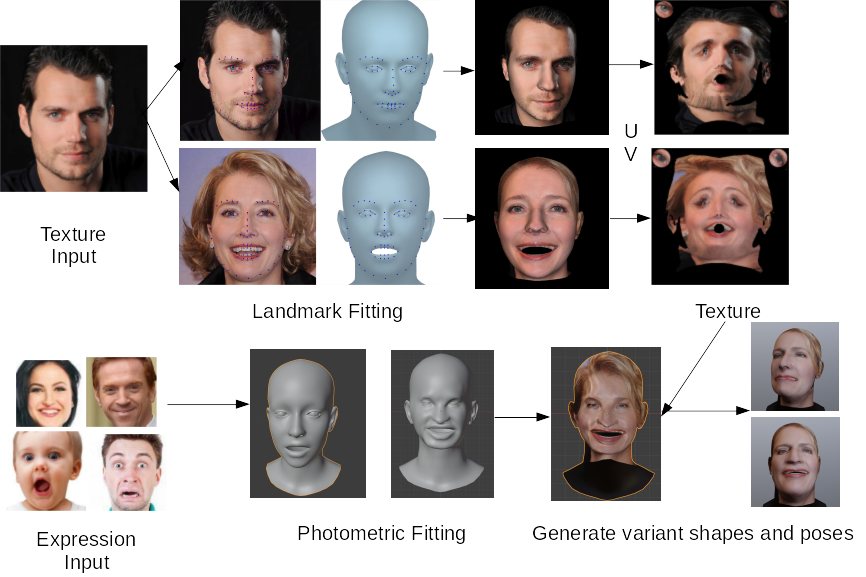
\includegraphics[width=\textwidth]{./figs/approach.png}
    \caption{Overview of our engine.On the top, we minimize landmark distance to extract the texture from the high resolution image. On the bottom, we extract the face models corresponding to different expressions by minimizing the photometric error, and then put the extracted texture onto the face models. Finally modify the weight of the blendshape to achieve different shape and pose with given facial expression. }
    \label{fig:approach}
\end{figure}

We first briefly introduce the setting of 3D morphable face model in section \ref{sec:3D}. Then, we explain how to use 3D facial model to generate faces, texture, and expression in section \ref{sec:face} and \ref{sec:expression}. Finally, we build a tools based on Blender \citep{blender} to generate synthetic data in section \ref{sec:data_generation}.

\section{3D Morphable Face Model Setting}
\label{sec:3D}
According to our introduction of relevant background knowledge in Chapter \ref{cha:background}, we tried different public available 3D morphable face model.

At first, we experimented the possibility of utilization the 3D Basel Face Model (BFM) \citep{bfm09}. Although BFM is the most widely used in academic research, we found that if we want to apply the model to facial expression generation, we need plenty of 3d scans mesh to generate blendshape for facial expressions. That means if we want to obtain a accurate expression blendshape, we need a lot of training data. And the model has 53490 vertices, it will take to much time to conduct an experiment on a general PC. 

Then, we measured the possibility of Facewarehouse \citep*{10.1109/TVCG.2013.249}. As shown in Figure \ref{fig:facewarehouse}, Facewarehouse has included 46 facial expression blendshapes, which will save a lot of time for modeling. However, we found that the blendshapes in the dataset was provided separately, and the order of each vertex was also inconsistent, so a lot of model rigging work demanded.

\begin{figure}[H]
    \centering
    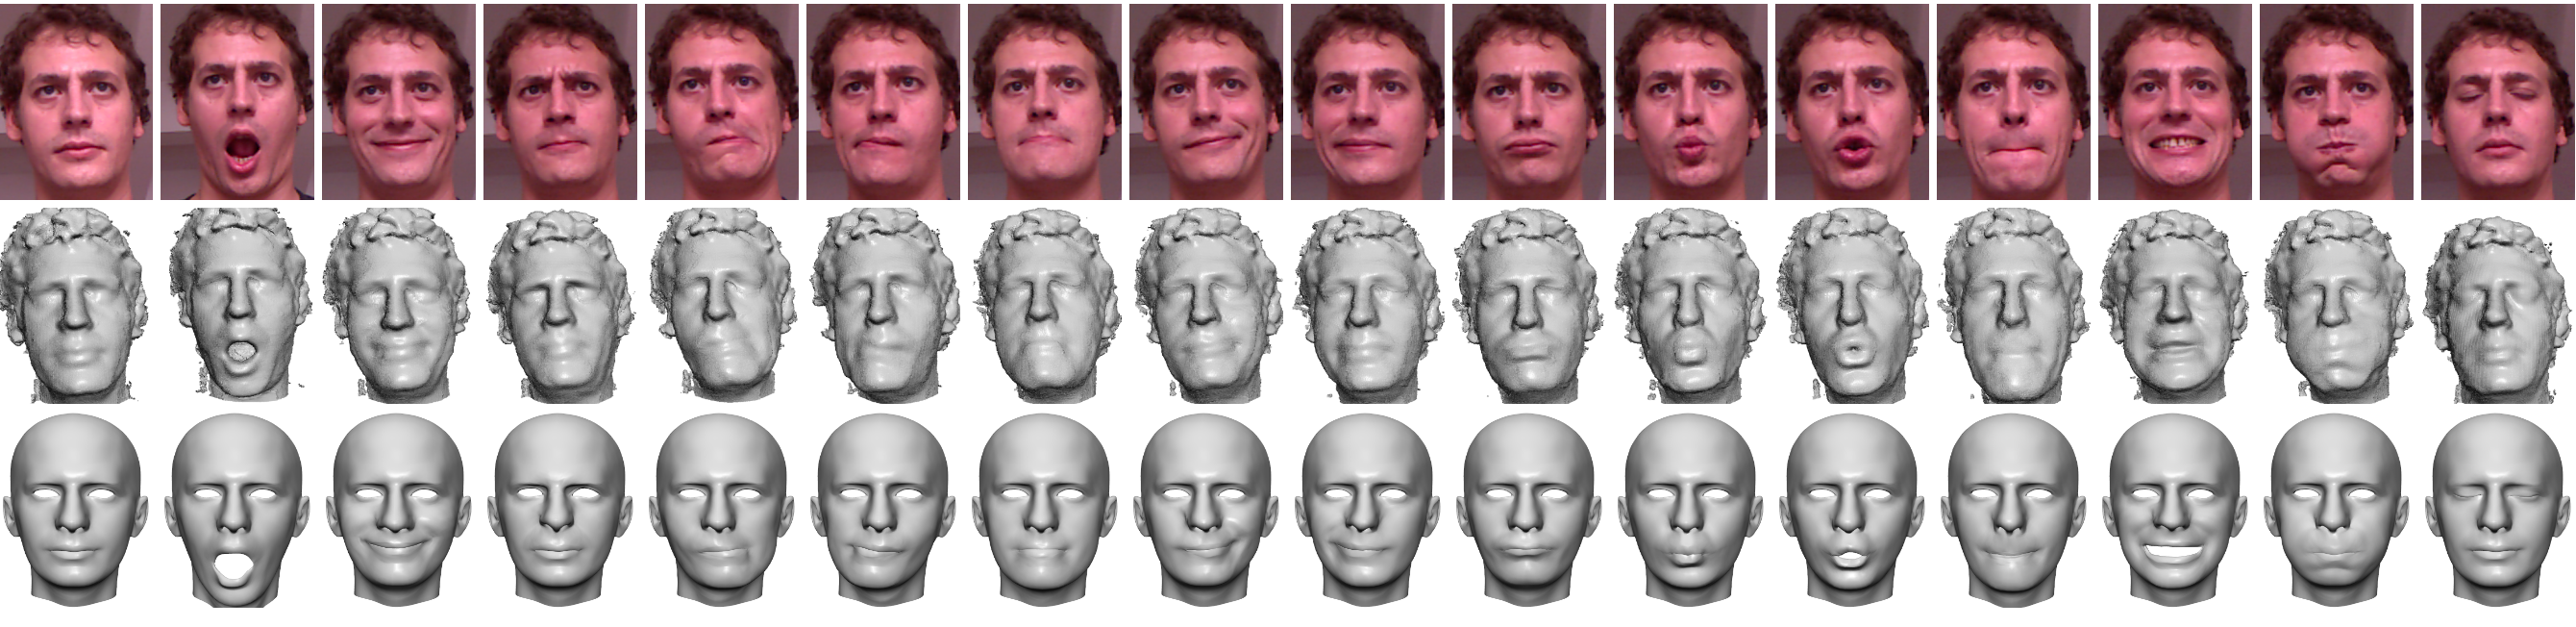
\includegraphics[width=\textwidth]{./figs/facewarehouse.png}
    \caption{Examples from Facewarehouse dataset }
    \label{fig:facewarehouse}
\end{figure}

Finally, after a few weeks of experimentation, we chose to use Faces Learned with an Articulated Model and Expressions (FLAME) \citep{flame}. Because this is a lightweight (only 5023 vertices), riging (vertics order fixed) face model. The author also provides 3D mesh static and dynamic 3d landmark. This means that we only need a projection matrix to generate the 2d landmarks of the 3d model.

\begin{figure}[H]
    \centering
    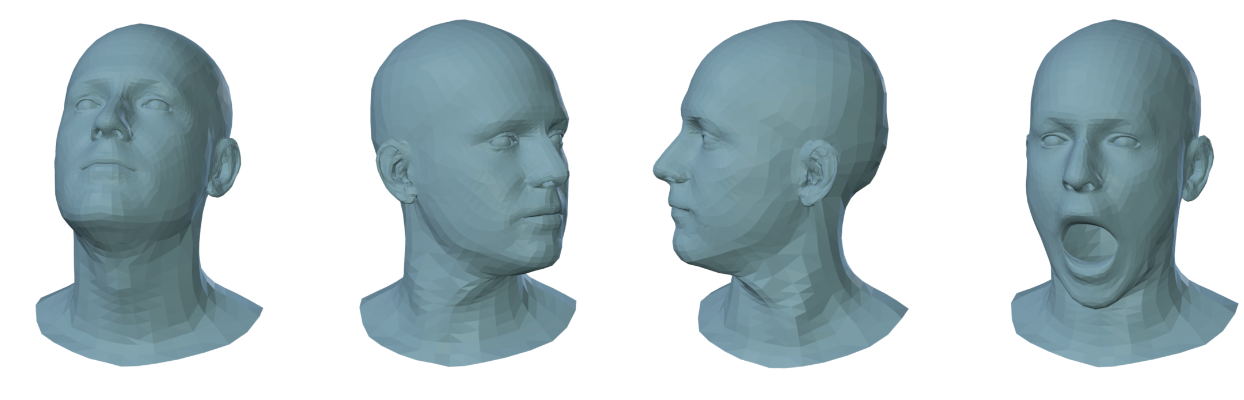
\includegraphics[width=\textwidth]{./figs/flame.png}
    \caption{Different pose examples from FLAME.}
    \label{fig:flame}
\end{figure}

\section{Face Model}
\label{sec:face}
This section will introduce some technical details. A face model usually consists of two components: \textbf{shape} and \textbf{texture}. With development of 3D modeling technology, we could  generate of different identities and expressions by adjusting the parameters of shape and texture. 

\textbf{Shape Model:} We use linear combination to describe the shape parameters. FLAME could be formulate a function \ref{eq:flame}:

\begin{equation}
    M(\vec{s} ,\vec{p} ,\vec{e}) :\mathbb{R}^{| \vec{s}| \times | \vec{p}| \times | \vec{e}| } \shortrightarrow \ \mathbb{R}^{3N}
    \label{eq:flame}
\end{equation}

where $N=5023$ vertices, shape coefficients: $\vec{s} \in \ \mathbb{R}^{| \vec{s}| }$,pose coefficients: $\vec{p} \in \ \mathbb{R}^{| \vec{p}| }$,expression coefficientss: $\vec{e} \in \ \mathbb{R}^{| \vec{e}| }$. Because, we have fixed the order of vertices, so we could perform Principal Component Analysis (PCA). The shape could be consist of the mean shape vector $\bar{M}$ and the linear combination of  

\section{Expression Model}
\label{sec:expression}


\section{Data Generation}
\label{sec:data_generation}